\documentclass[a4paper]{scrreprt}
\usepackage[T1]{fontenc}
\usepackage[utf8]{inputenc}
\usepackage[ngerman]{babel}
\usepackage{graphicx}

\usepackage[
	colorlinks=true,
	urlcolor=blue,
	linkcolor=black
]{hyperref}

\begin{document}
\title{Projekt A - Einführung in das Programmieren~\\ 
\vspace{\fill}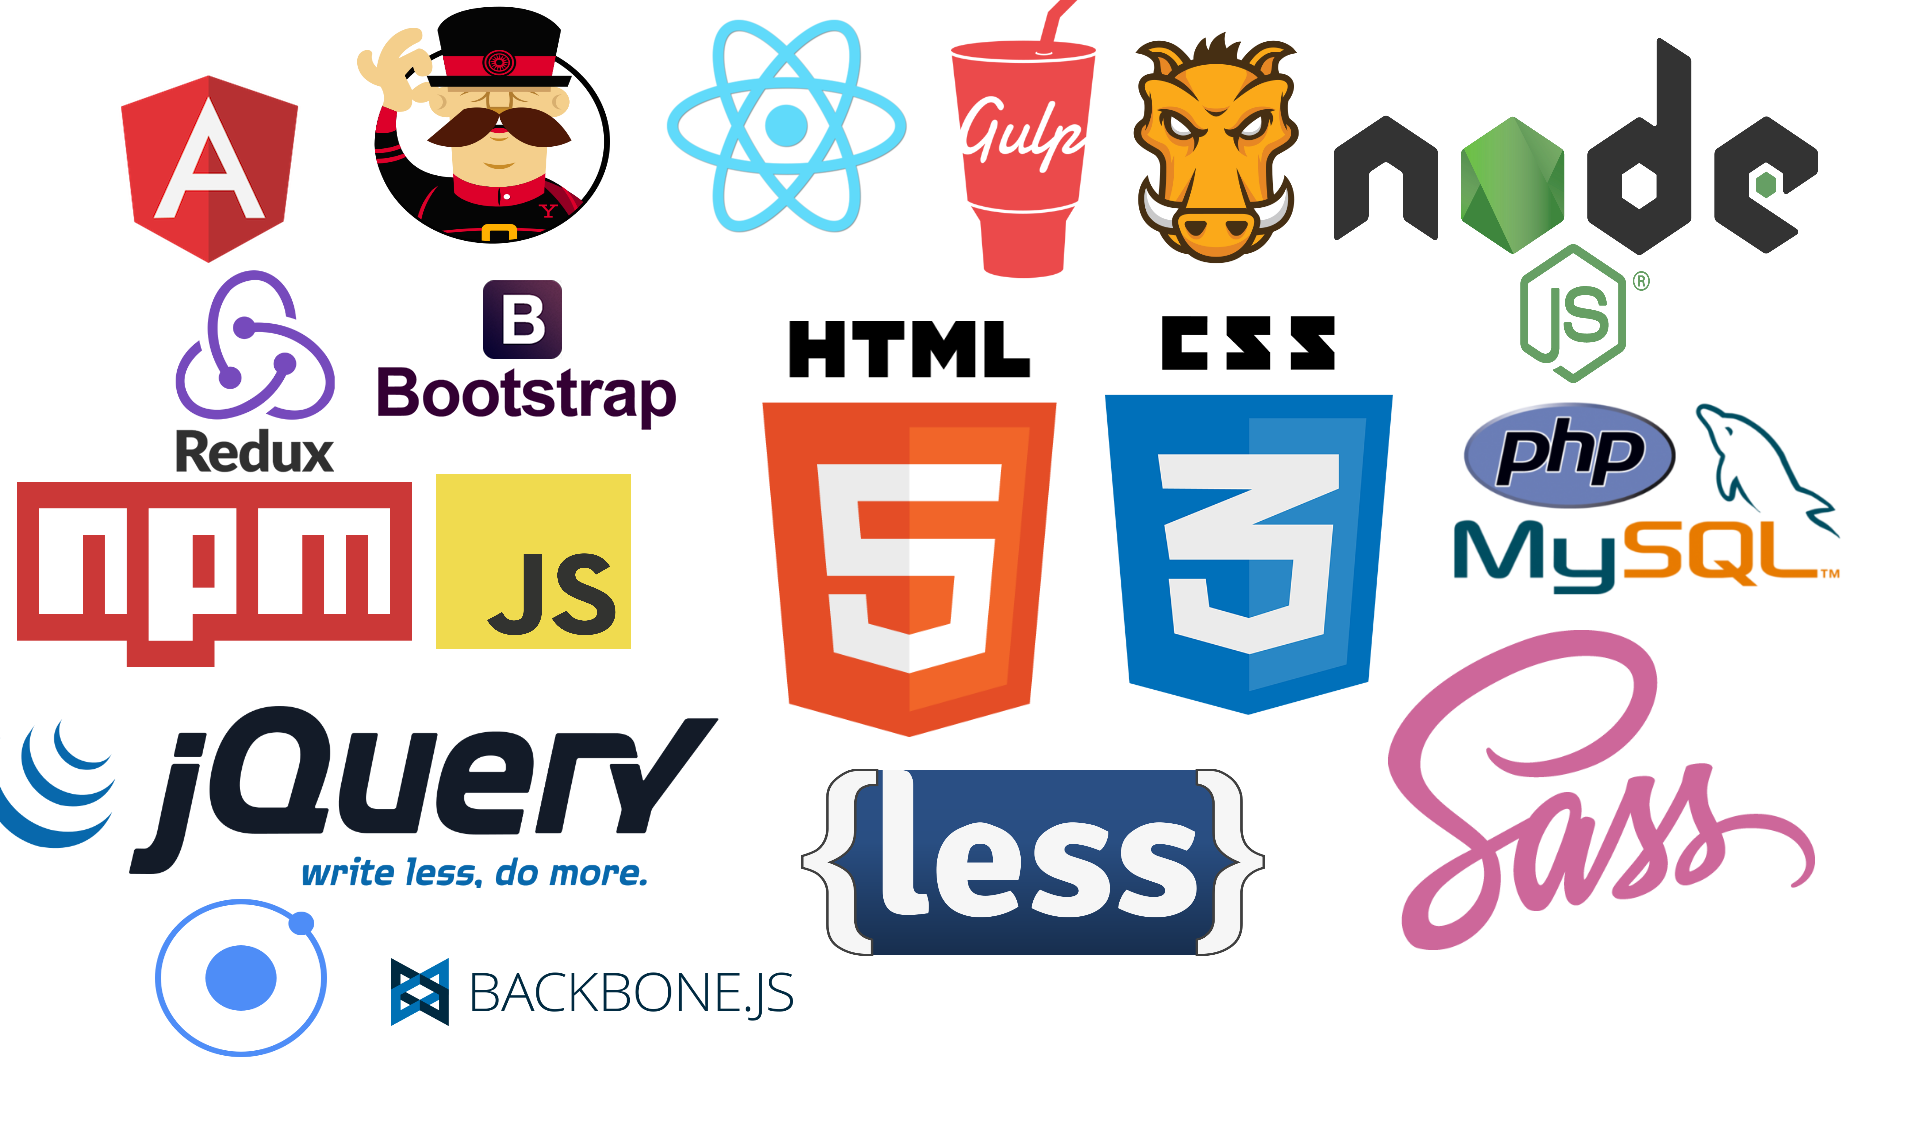
\includegraphics[scale=0.2]{collage_web}}
\author{Tim Zschage u. Florian Wiekhorst \textsc{Student}\\ Prof. Dr. Andreas Plaß~ \textsc{Lehrender}}
\publishers{HAW Hamburg}
\date{5.1.2017}
\maketitle
\tableofcontents
\newpage
\chapter{Projektidee nach Alpers}

\section{Einleitung}
Für mein Projekt möchte ich das Brettspiel Kingsburg als webbasierte Anwendung umsetzen.
Das Ziel des Spiels Kingsburg ist, sein Königreich mit neuen Gebäuden aufzubauen und mithilfe seiner Berater seine Armee so zu verstärken, dass man am Ende jedes Jahres gegen einen Feind gewinnen kann. Es gibt 5 Jahre mit jeweils 7 Phasen. Am Ende jedes Jahres kämpfen die Spieler gegen einen Gegner der bei einem Sieg einen Bonus, bei einer Niederlage einen Malus einbringt.
Am Ende gewinnt derjenige mit den meisten Punkten.


\section{Phase 1(Spielbeginn):}

Das Spiel beginnt in Phase 1 des ersten Jahres.
Jeder Spieler darf sich drei zufällige Zahlen ausgeben lassen.

Relevant ab Jahr 2:
In der ersten Phase kann sich der Spieler, mit den wenigsten Gebäuden eine zusätzliche Zahl ausgeben lassen.

\section{Phase 2(Produktionsphase):}

In der Produktionsphase werden zufällige Werte zwischen 1 und 6 generiert.

Auf dem Spielfeld gibt es 18 königliche Berater, die einem Vorteile bringen. Die Berater geben entweder Punkte, einen Rohstoff (Gold,Holz,Stein) der zum Bauen von Gebäuden notwendig ist, militärische Stärke oder einen "+2 Token", welcher eingesetzt werden kann um die zufällig generierten Werte zu erhöhen. Jeder Spieler kann nun einen Berater für sich beanspruchen, der einer der zufällig generierten Zahlen entspricht. Die in Frage kommenden Berater werden je nach zufällig generierter Zahl angezeigt und man muss sich entscheiden. Der Spieler mit der geringsten zufällig generierten Zahl darf als erstes einen Berater wählen. Ein Berater kann nur einmal belegt werden. Am Ende müssen entweder alle drei zufällig generierten Zahlen auf die Berater verteilt sein, oder es sind schon alle möglichen Berater belegt.

Jeder Spieler kann nun mit Ressourcen ein Gebäude bauen, welche in einer festen Reihenfolge vorliegen. Die Gebäude sind nicht Spielerabhängig. Jedes Gebäude bringt Punkte und einen einzigartigen Bonus. Die verfügbaren Gebäude werden einem angezeigt. Ist ein Gebäude nicht verfügbar weil man das vorherige Gebäude nicht gebaut hat, so wird es einem auch nicht angezeigt.


\section{Phase 3:}

In Phase 3 kriegt der Spieler, mit den meisten Gebäuden einen Bonuspunkt hinzu.


\section{Phase 4(Produktionsphase):}

siehe Phase 2.

\section{Phase 5:}

In Phase 5 kriegt der Spieler, mit den wenigsten Gebäuden, bei Gleichstand der Spieler mit den wenigsten Ressourcen, einen Gesandten zugeteilt.
Herrscht Gleichstand sowohl bei Gebäuden als auch bei Ressourcen kriegt keiner den Gesandten.

Dieser Gesandte kann während jeder Produktionsphase für eine von zwei Aktionen verwendet werden:

a) Ein Berater, der schon belegt wurde von einem selbst oder einem anderen Spieler kann ein weiteres Mal belegt werden. Es müssen jedoch trotzdem die zufällig generierten Zahlen zwischen 1 und 6 benutzt werden

b) Während der Konstruktionsphase der Gebäude, dürfen zwei Gebäude gebaut werden. Es müssen jedoch für beide Gebäude die Ressourcen bezahlt werden

Wird der Gesandte bis zur Phase 5 des nächsten Jahres nicht benutzt wird er erneut vergeben.


\section{Phase 6(Produktionsphase):}

s.o.


\section{Phase 7:}

In dieser Phase haben Spieler die Möglichkeit, zwei beliebige Ressourcen gegen einen Militärpunkt einzutauschen.


\section{Phase 8(Jahresende):}

Am Ende des Jahres spawnt ein zufälliger Gegner gegen den gekämpft wird.
Nun kommt es auf die Militärpunkte an.
Zunächst wird eine zufällige Zahl zwischen 1 und 6 generiert, die bestimmt, wieviele Militärpunkte der König jedem Spieler zusätzlich gibt.
Nun wird geguckt wie stark der Gegner ist, was variieren kann. In Jahr 1 haben die Gegner 2 - 4 Stärkepunkte und von Jahr zu Jahr werden die Gegner stärker.
Hat man also mehr Militärpunkte als der Gegner, so kriegt man einen Bonus bzw. einen Malus wenn man weniger Punkte hat als der Gegner.
Dieser Malus kann entweder der Verlust von Punkten sein, der Verlust von Ressourcen, oder man muss sein stärkstes Gebäuden zerstören.

Nach dieser Phase fängt das nächste Jahr an.
Am Ende des 5.Jahres gewinnt der Spieler mit den meisten Punkten.


\section{Für 1 Spieler:}

Das Spiel ist zwar als Multiplayerspiel konzipiert, bietet jedoch eine Art Arcade Modus für Einzelspieler.
Der Modus ist darauf ausgelegt seine Armee über 4 Runden so aufzubauen, dass in der 5. Phase, der Kampfesphase, man stark genug ist um den Gegner zu besiegen.
Ziel ist es, 3 Wellen von á 5 Gegnern zu überstehen.
Der 5. Gegner ist jeweils ein Boss und stärker als die vorherigen Gegner.

Die Phasen 1-3 entsprechen den normalen Produktionsphasen.
Die 4. Phase entspricht der Rekrutierungsphase, während der man gegen Rohstoffe seine Armee verstärken kann.
Im Arcademodus soll es jedoch so sein, dass man sich entscheiden soll, ob man Rohstoffe bezahlt um neue Soldaten zu kriegen, oder ob man seine Rohstoffe behält und selber in den Kampf zieht.
Ist dies der Fall, bleibt die Kampfstärke wie sie ist und man kriegt zwei beliebige Rohstoffe für die nächste Runde hinzu.
Phase 5 ist der Kampf. Die Gegner werden von Welle zu Welle stärker und alle 5 Runden gibt es einen Bosskampf, der nochmal signifikant stärker ist.

Übersteht man alle 15 Runden, so hat man gewonnen.

\chapter{Installationsanleitung}
Um "`Kingsburg"' spielen zu können, ist die Installation eines lokalen Webservers erforderlich. Wir verwenden für unsere Zwecke die Apache-Distribution XAMPP. Der "`Apache HTTP Server"' ist der Name eines freien Webservers. 

\section{XAMPP}
\href{https://www.apachefriends.org/de/index.html}{www.apachefriends.org/de/index.html}

Nach dem Download und der anschließenden Installation des Webservers sollte sich nun ein Ordner mit dem Namen "`xampp"' im C: Verzeichnis befinden. Dieser Ordner hat einen Unterordner der "`htdocs"' heißt. In diesen Ordner wird nun der Projektordner hinein gezogen. \\
Bevor man nun auf den Ordner über den Browser zugreifen kann muss zunächst der Webserver, sowie der mitgelieferte MySQL-Server, über das XAMPP Control Panel gestartet werden. Wir benötigen MySQL um unsere Datenbank für das Spiel einzurichten. \\
Auf den XAMPP Server zugegriffen wird über den Browser:\\

\includegraphics[scale=0.8]{browser_localhost}\\
Der Bezeichner "`localhost"' bezieht sich auf die Home IP-Adresse 127.0.0.1 eines Servers. Will ein externer Rechner auf den Server zugreifen so muss "`localhost"' bzw. 127.0.0.1 durch die jeweilige Rechner IPv4-Adresse ersetzt werden.
Seine IP-Adresse kann man durch den Befehl "`ipconfig"' im Kommandozeilenfenster herausfinden:\\
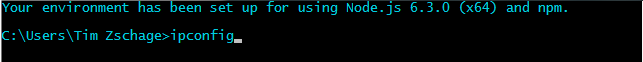
\includegraphics[scale=0.8]{ipconfig}\\
\linebreak
Es kann durchaus vorkommen, dass ein anderes Programm den Standardport 80 blockiert. 
Über das XAMPP Control Panel kann die Konfigurationsdatei, "`httpd.conf"', des Servers aufgerufen und der Port von 80 auf beispielsweise 8080 geändert werden.
Jetzt ist es jedoch notwendig den Port hinter localhost zu schreiben:\\

\includegraphics[scale=0.8]{browser_port}\\

\chapter{Systemarchitektur}
Unsere Webanwendung ist gedacht als Client-Server Kommunikation. Beispielsweise bei dem Registrier/Login Vorgang schickt der User eine Datenbankanfrage an den Server und der Server speichert entweder die eingegebenen Daten oder vergleicht sie um den User einzuloggen.\\
Bei dem Spiel ist es angedacht, durch Ajax-Anfragen an den Server die Clientseitigen Elemente stetig zu ändern, wie zum Beispiel die Punktestände oder das Inventar der Spieler.\\
Komplett Clientseitig sind lediglich die Menüs mit den Links zum Impressum bzw. der Spielwebsite.

\end{document}